\documentclass[12pt]{article}
\usepackage[margin = 0.9in, top=0.8in]{geometry}
\usepackage{graphicx}
\usepackage{textgreek}
\usepackage{amsmath}
\usepackage{amsfonts}
\usepackage{mathtools}
\usepackage{amssymb}
\usepackage{float}
\usepackage{subcaption}
\usepackage{hyperref}
\usepackage{grffile}
\graphicspath{{./2/images},{./}}

\title{CS 754 - Advanced Image Processing\\Assignment 2 - Report}
\author{Shaan ul Haque - 180070053\\Mantri Krishna Sri Ipsit - 180070032}
\newcommand{\norm}[1]{\left\lVert #1 \right\rVert}
\newcommand{\R}{\mathbb{R}}
\begin{document}

\maketitle

\section*{Question 1}
\subsection*{1.1}
If $\delta_{2s} = 1$, then for any $2s$ - sparse vector $h \in \R^n$, we have
\begin{equation}
0 \leq \norm{\Phi h}_2^2 \leq 2\: \norm{h}_2^2
\end{equation}
If $2s$ columns of $\Phi$ are linearly dependent, then we have
$$\sum_i \alpha_i \phi_i = 0 \:\:\:, \alpha_i \neq0$$
Where $\{\phi_i\}$ are the $2s$ linearly dependent columns of $\Phi$ and $\{\alpha_i\}$ are some non-zero constants. This summation can be re-written as
$$\Phi v = 0, \:\:\: \Phi = [\phi_1| \ldots |\phi_{2s}], v^{\text{T}} = [\alpha_1, \ldots, \alpha_{2s}]$$
Now, we can extend $v$ by adding rows of zeros so that the extended vector $v_1 \in \R^n$. Similarly, we can extend the columns of $\Phi$ by adding random columns (this works because we want the measurement matrix to be random in Compressed Sensing) so that $\Phi \in \R^{m \times n}$. Even after this extension, we still have
$$\Phi v_1 = 0$$
Clearly, we can see that $v_1$ is a $2s$ - sparse vector and also satisfies (1) trivially because $\norm{\Phi v_1}_2 = 0$.
Hence, the above justifies that when $\delta_{2s} = 1$, there exists a $2s$ - sparse vector $h$ such that $\Phi h = 0$ and $2s$ columns of $\Phi$ are linearly dependent.  
\subsection*{1.2}
We have $x^*$ and $x$ which satisfy the convex optimization problem
\begin{equation}
\min _{\tilde{x}\in \R^n} \norm{\tilde{x}}_1 \:\:\: \text{ subject to } \norm{y - \Phi \tilde{x}}_2 \leq \epsilon
\end{equation}
Consider
$$\norm{\Phi(x^* - x)}_2 = \norm{(\Phi x^* - y) + (y - \Phi x)}_2$$
Then, using the triangle inequality, we have
$$\norm{\Phi(x^* - x)}_2 = \norm{(\Phi x^* - y) + (y - \Phi x)}_2 \leq \norm{\Phi x^* - y}_2 + \norm{y-\Phi x}_2$$
But using (2) we can say that
$$\norm{\Phi x^* - y}_2 + \norm{y-\Phi x}_2 \leq \epsilon + \epsilon = 2\epsilon$$
Hence, we have
$$\norm{\Phi(x^* - x)}_2 \leq \norm{\Phi x^* - y}_2 + \norm{y-\Phi x}_2 \leq 2\epsilon$$
\subsection*{1.3}
We know that each $h_{T_j}$ is $s$ sparse. We also know that the $\ell_{\infty}$ norm of a vector denotes the maximum element of that vector. As $h_{T_j}$ is $s$ sparse, we have, for each non-zero entry $\alpha_i$ of $h_{T_j}$
$$\alpha_i^2 \leq \norm{h_{T_j}}_{\infty}^2 \:\:\: i = 1, 2, 3, \ldots, s$$
Adding all the above $s$ inequalities, we have
$$\norm{h_{T_j}}_2^2 \leq s \: \norm{h_{T_j}}_{\infty}^2$$
\begin{equation}
	\implies \norm{h_{T_j}}_2 \leq s^{1/2} \: \norm{h_{T_j}}_{\infty}
\end{equation}
We know that, by the construction of the vectors $\{h_{T_j}\}$, the largest element of $h_{T_j}$ is smaller than the smallest element of $h_{T_{j-1}}$. In fact, the $\norm{h_{T_j}}_{\infty}$ is smaller than every (non-zero) element of $h_{T_{j-1}}$. Re-writing this mathematically, we have
$$\norm{h_{T_j}}_{\infty} \leq |\beta_i| \:\:\: i = 1, 2, 3, \ldots, s$$
Adding all the above $s$ inequalities, we get
$$s\: \norm{h_{T_j}}_{\infty} \leq \norm{h_{T_{j-1}}}_{1}$$
\begin{equation}
\implies s^{1/2}\: \norm{h_{T_j}}_{\infty} \leq  s^{-1/2} \:\norm{h_{T_{j-1}}}_{1}
\end{equation}
Combining the inequalities (3) and (4), we have
$$\norm{h_{T_j}}_2 \leq s^{1/2} \: \norm{h_{T_j}}_{\infty} \leq  s^{-1/2} \:\norm{h_{T_{j-1}}}_{1}$$
\subsection*{1.4}
Using the relation between the 1st and the 3rd expression in the above inequality, we have
$$\norm{h_{T_j}}_2 \leq s^{-1/2} \:\norm{h_{T_{j-1}}}_{1}$$
Summing up all such above inequalities for $j \geq 2$, we have
\begin{equation}
\sum \limits_{j \geq 2} \norm{h_{T_j}}_2 \leq s^{-1/2} \: \bigg(\norm{h_{T_1}}_1 + \norm{h_{T_2}}_1 + \ldots\bigg)
\end{equation}
By construction of $\{h_{T_{j}}\}$, we can say that 
$$\norm{h_{T_1}}_1 + \norm{h_{T_2}}_1 + \ldots = \norm{h_{T_0^c}}_1$$ 
Hence, (5) becomes
\begin{equation}
\sum \limits_{j \geq 2} \norm{h_{T_j}}_2 \leq s^{-1/2} \: \bigg(\norm{h_{T_1}}_1 + \norm{h_{T_2}}_1 + \ldots\bigg) \leq s^{-1/2} \:\norm{h_{T_0^c}}_1
\end{equation}
\subsection*{1.5}
We know that 
$$h_{(T_0 \cup T_1)^c} = \sum_{j \geq 2} h_{T_j}$$
Hence, we have
$$\norm{h_{(T_0 \cup T_1)^c}}_2 = \norm{\sum_{j \geq 2} h_{T_j}}_2$$
Using the extended version of triangle inequality for the above equation and using the inequality (6) above,  we get
\begin{equation}
	\norm{h_{(T_0 \cup T_1)^c}}_2 = \norm{\sum_{j \geq 2} h_{T_j}}_2 \leq \sum_{j \geq 2} \norm{h_{T_j}}_2 \leq s^{-1/2} \:\norm{h_{T_0^c}}_1
\end{equation}
\subsection*{1.6}
We have the \textit{reverse triangle inequality} for any two real numbers as follows:
$$|x - y| \geq \bigg||x| - |y|\bigg|$$
Using this inequality for $|x_i + h_i|, i \in T_0$, we have
$$|x_i + h_i| \geq \bigg||x_i| - |h_i|\bigg| \geq |x_i| - |h_i|$$
Summing over all $i \in T_0$, we have
\begin{equation}
\sum \limits_{i \in T_0}|x_i + h_i| \geq \norm{x_{T_0}}_1 - \norm{h_{T_0}}_1
\end{equation}
Again using the reverse triangle inequality for $|h_i + x_i|, i \in T_0^c$, we have
$$|h_i + x_i| \geq \bigg||h_i| - |x_i|\bigg| \geq |h_i| - |x_i|$$
Summing over all $i \in T_1$, we have
\begin{equation}
\sum \limits_{i \in T_0^c}|x_i + h_i| \geq \norm{h_{T_0^c}}_1 - \norm{x_{T_0^c}}_1
\end{equation}
By adding the inequalities (8) and (9) we get
\begin{equation}
	\sum \limits_{i \in T_0}|x_i + h_i| + \sum \limits_{i \in T_0^c}|x_i + h_i| \geq \norm{x_{T_0}}_1 - \norm{h_{T_0}}_1 + \norm{h_{T_0^c}}_1 - \norm{x_{T_0^c}}_1
\end{equation}
\subsection*{1.7}
As per the convex optimization problem that we are solving, we have
$$\norm{x}_1 \geq \norm{x + h}_1$$
Using this in the inequality (10) we have
\begin{equation}
	\norm{x}_1 \geq \norm{x_{T_0}}_1 - \norm{h_{T_0}}_1 + \norm{h_{T_0^c}}_1 - \norm{x_{T_0^c}}_1
\end{equation}
By definition we have
$$\norm{x_{T_0^c}}_1 = \norm{x - x_s}_1$$
By using the reverse triangle inequality, we have
$$\norm{x_{T_0^c}}_1 = \norm{x - x_s}_1 \geq \norm{x}_1 - \norm{x_s}_1$$
Noting the fact that $\norm{x_s} = \norm{x_{T_0}}$ and using inequality (11) we have
$$\norm{x_{T_0^c}}_1 \geq \norm{x_{T_0}}_1 - \norm{h_{T_0}}_1 + \norm{h_{T_0^c}}_1 - \norm{x_{T_0^c}}_1 - \norm{x_{T_0}}_1$$
which is same as
\begin{equation}
\norm{h_{T_0^c}}_1 \leq \norm{h_{T_0}}_1 + 2\,\norm{x_{T_0^c}}_1
\end{equation}
\subsection*{1.8}
Using inequalities (7) and (12) we have
$$\norm{h_{(T_0 \cup T_1)^c}}_2 \leq s^{-1/2} \bigg(\norm{h_{T_0}}_1 + 2\,\norm{x_{T_0^c}}_1\bigg)$$
Using the known inequality $\norm{v}_1 \leq \sqrt{k} \, \norm{v}_2$ for a $k$ sparse vector v, we have
$$\norm{h_{(T_0 \cup T_1)^c}}_2 \leq s^{-1/2} \bigg(\norm{h_{T_0}}_1 + 2\,\norm{x_{T_0^c}}_1\bigg) \leq s^{-1/2} \bigg(\sqrt{s}\, \norm{h_{T_0}}_2 + 2\, \norm{x_{T_0^c}}_1\bigg)$$
Hence we have
\begin{equation}
	\norm{h_{(T_0 \cup T_1)^c}}_2 \leq \norm{h_{T_0}}_2 + 2e_0, \:\:\: e_0 \equiv s^{-1/2}\, \norm{x - x_s}_1
\end{equation}
\subsection*{1.9}
We know that by Cauchy-Schwartz inequality, we have
\begin{equation}
|\langle \Phi h_{T_0 \cup T_1}, \Phi h\rangle| \leq \norm{\Phi  h_{T_0 \cup T_1}}_2 \, \norm{\Phi h}_2
\end{equation}
As $h = x^* - x$, we have by inequality justified in section 1.3, 
$$\norm{\Phi h}_2 = \norm{\Phi (x^* - x)}_2 \leq 2\epsilon$$
also, as $h_{T_0 \cup T_1}$ is a $2s$ sparse vector and $\Phi$ follows RIP of order $2s$, we have
$$\norm{\Phi h_{T_0 \cup T_1}}_2 \leq \sqrt{1 + \delta_{2s}} \, \norm{ h_{T_0 \cup T_1}}_2$$
Using the above two inequalities in (14), we have
\begin{equation}
	|\langle \Phi h_{T_0 \cup T_1}, \Phi h\rangle| \leq \norm{\Phi  h_{T_0 \cup T_1}}_2 \, \norm{\Phi h}_2 \leq 	2\epsilon \sqrt{1 + \delta_{2s}} \, \norm{ h_{T_0 \cup T_1}}_2
\end{equation}
\subsection*{1.10}
Lemma 2.1 from the paper states
$$|\langle \Phi x, \Phi x' \rangle | \leq \delta_{s + s'}\, \norm{x}_2 \norm{x'}_2$$
for all $x, x'$ supported on disjoint subsets $T, T' \subset \{1, 2, \ldots, n\}$ with $|T| \leq s, |T'| \leq s'$
Using this lemma for $x = h_{T_0}$ and $x' = h_{T_j}$, we have
\begin{equation}
|\langle \Phi h_{T_0}, \Phi h_{T_j}\rangle | \leq \delta_{2s} \, \norm{h_{T_0}}_2 \norm{h_{T_j}}_2
\end{equation}
\subsection*{1.11}
We know that for two positive real numbers $a$ and $b$, the QM-AM inequality is as follows:
$$\frac{a + b}{2} \leq \sqrt{\frac{a^2 + b^2}{2}}$$
Taking $a = \norm{h_{T_0}}_2$ and $b = \norm{h_{T_1}}_2$ and substituting in the above inequality, we get
\begin{equation}
\norm{h_{T_0}}_2 + \norm{h_{T_1}}_2 \leq \sqrt{2} \:\sqrt{\norm{h_{T_0}}_2^2 + \norm{h_{T_1}}_2^2} = \sqrt{2}\, \norm{h_{T_0 \cup T_1}}_2
\end{equation}
as $T_0$ and $T_1$ are disjoint.
\subsection*{1.12}
By replacing $T_0$ with $T_1$ in inequality (16) and adding both, we get
$$|\langle \Phi h_{T_0}, \Phi h_{T_j}\rangle | + |\langle \Phi h_{T_1}, \Phi h_{T_j}\rangle | \leq \delta_{2s} (\norm{h_{T_0}}_2 + \norm{h_{T_1}}_2) \norm{h_{T_{j}}}$$
Making use of triangle inequality for the LHS of above inequality, we get
$$|\langle \Phi h_{T_0} + \Phi h_{T_1}, \Phi h_{T_j}\rangle | \leq \delta_{2s} (\norm{h_{T_0}}_2 + \norm{h_{T_1}}_2) \norm{h_{T_{j}}}$$
Replacing $\Phi h_{T_0} + \Phi h_{T_1} = \Phi h_{T_0 \cup T_1}$ and above inequalities for $j \geq 2$, we get
$$\sum \limits_{j \geq 2} |\langle \Phi h_{T_0 \cup T_1}, \Phi h_{T_j}\rangle |\leq \delta_{2s} (\norm{h_{T_0}}_2 + \norm{h_{T_1}}_2) \, \bigg(\sum \limits_{j \geq 2} \norm{h_{T_j}}_2\bigg)$$
Again making use of triangle inequality for the LHS of the above inequality, we get
$$\bigg|\bigg\langle \Phi h_{T_0 \cup T_1}, \sum_{j \geq 2} \Phi h_{T_j}\bigg\rangle \bigg| \leq \delta_{2s} (\norm{h_{T_0}}_2 + \norm{h_{T_1}}_2) \, \bigg(\sum \limits_{j \geq 2} \norm{h_{T_j}}_2\bigg)$$
Finally, using (17), we finally have
\begin{equation}
\bigg|\bigg\langle \Phi h_{T_0 \cup T_1}, \sum_{j \geq 2} \Phi h_{T_j}\bigg\rangle \bigg| \leq \delta_{2s} \, \sqrt{2}\,\norm{h_{T_0 \cup T_1}} \, \bigg(\sum \limits_{j \geq 2} \norm{h_{T_j}}_2\bigg)
\end{equation}
Now, using the fact that $\Phi h = \Phi h_{T_0 \cup T_1} + \sum_{j \geq 2} \Phi h_{T_j}$ in the inequality (15) above, we get
$$\bigg|\bigg\langle \Phi h_{T_0 \cup T_1}, \Phi h_{T_0 \cup T_1} + \sum_{j \geq 2} \Phi h_{T_j}\bigg\rangle \bigg| \leq 	2\epsilon \sqrt{1 + \delta_{2s}} \, \norm{ h_{T_0 \cup T_1}}_2$$
Using the linearity property of inner product, we have
\begin{equation}
	\bigg|\norm{\Phi h_{T_0 \cup T_1}}_2^2 + \bigg\langle \Phi h_{T_0 \cup T_1}, \sum_{j \geq 2} \Phi h_{T_j}\bigg\rangle \bigg| \leq 	2\epsilon \sqrt{1 + \delta_{2s}} \, \norm{ h_{T_0 \cup T_1}}_2
\end{equation}
Now, adding the inequalities (18) and (19), we get
\begin{eqnarray*}
\bigg|\norm{\Phi h_{T_0 \cup T_1}}_2^2 + \bigg\langle \Phi h_{T_0 \cup T_1}, \sum_{j \geq 2} \Phi h_{T_j}\bigg\rangle \bigg| + \bigg|\bigg\langle \Phi h_{T_0 \cup T_1}, \sum_{j \geq 2} \Phi h_{T_j}\bigg\rangle \bigg| &\leq& 	2\epsilon \sqrt{1 + \delta_{2s}} \, \norm{ h_{T_0 \cup T_1}}_2 + \\ 
&& \delta_{2s} \, \sqrt{2}\,\norm{h_{T_0 \cup T_1}} \, \bigg(\sum \limits_{j \geq 2} \norm{h_{T_j}}_2\bigg)
\end{eqnarray*}
We know from the triangle inequality that 
$$\norm{\Phi h_{T_0 \cup T_1}}_2^2 \leq \bigg|\norm{\Phi h_{T_0 \cup T_1}}_2^2 + \bigg\langle \Phi h_{T_0 \cup T_1}, \sum_{j \geq 2} \Phi h_{T_j}\bigg\rangle \bigg| + \bigg|- \bigg\langle \Phi h_{T_0 \cup T_1}, \sum_{j \geq 2} \Phi h_{T_j}\bigg\rangle \bigg|$$
Using this, we finally have,
\begin{equation}
\norm{\Phi h_{T_0 \cup T_1}}_2^2 \leq \norm{ h_{T_0 \cup T_1}}_2 \, \bigg(2\epsilon \sqrt{1 + \delta_{2s}} + \sqrt{2}\,\delta_{2s}\,\sum \limits_{j \geq 2} \norm{h_{T_j}}_2\bigg)
\end{equation}
From the restricted isometry property, we have
$$(1 - \delta_{2s})\, \norm{h_{T_0 \cup T_1}}_2^2 \leq \norm{\Phi h_{T_0 \cup T_1}}_2^2$$
Hence, we have
\begin{equation}
(1 - \delta_{2s})\, \norm{h_{T_0 \cup T_1}}_2^2 \leq \norm{\Phi h_{T_0 \cup T_1}}_2^2 \leq
\norm{ h_{T_0 \cup T_1}}_2 \, \bigg(2\epsilon \sqrt{1 + \delta_{2s}} + \sqrt{2}\,\delta_{2s}\,\sum \limits_{j \geq 2} \norm{h_{T_j}}_2\bigg) 
\end{equation}
\subsection*{1.13}
By combining the inequality (6) with RHs of (21), we have
$$\norm{ h_{T_0 \cup T_1}}_2 \, \bigg(2\epsilon \sqrt{1 + \delta_{2s}} + \sqrt{2}\,\delta_{2s}\,\sum \limits_{j \geq 2} \norm{h_{T_j}}_2\bigg) \leq \norm{h_{T_0 \cup T_1}}_2 \bigg(2\epsilon \sqrt{1 + \delta_{2s}} + \sqrt{2}\delta_{2s} \, s^{-1/2} \norm{h_{T_0^c}}_1\bigg)$$
Using the above inequality with (21), we have
$$(1 - \delta_{2s})\norm{h_{T_0 \cup T_1}}_2^2 \leq \norm{h_{T_0 \cup T_1}}_2 \bigg(2\epsilon \sqrt{1 + \delta_{2s}} + \sqrt{2}\delta_{2s} \, s^{-1/2} \norm{h_{T_0^c}}_1\bigg)$$
On simplifying the above inequality, we get
\begin{equation}
\norm{h_{T_0 \cup T_1}}_2 \leq \alpha \epsilon + \rho s^{-1/2} \norm{h_{T_0^c}}_1, \:\:\: \alpha \equiv \frac{2 \sqrt{1 + \delta_{2s}}}{1 - \delta_{2s}}, \rho \equiv \frac{\sqrt{2}\delta_{2s}}{1 - \delta_{2s}}
\end{equation}
\subsection*{1.14}
We now conclude from (22) and (12) that 
$$\norm{h_{T_0 \cup T_1}}_2 \leq \alpha \epsilon + \rho s^{-1/2}\norm{h_{T_0}}_1 + 2\rho e_0 \leq \alpha \epsilon + \rho \norm{h_{T_0}}_2 + 2\rho e_0$$
As $T_0$ and $T_1$ are disjoint and $h_{T_0}$ and $h_{T_1}$ are both $s$ sparse, we can say that 
$$\norm{h_{T_0}}_2 \leq \norm{h_{T_0} + h_{T_1}}_2 = \norm{h_{T_0 \cup T_1}}_2$$
Using this in the above inequality, we get
$$\norm{h_{T_0 \cup T_1}}_2 \leq \alpha \epsilon + \rho \norm{h_{T_0 \cup T_1}}_2 + 2 \rho e_0$$
On simplifying, we get
\begin{equation}
\norm{h_{T_0 \cup T_1}}_2 \leq (1 - \rho)^{-1} \, (\alpha \epsilon + 2\rho e_0)
\end{equation}
\subsection*{1.15}
We can write $h$ as
$$h = h_{T_0 \cup T_1} + h_{(T_0 \cup T_1)^c}$$
Hence, by triangle inequality, we have
$$\norm{h}_2 \leq \norm{h_{T_0 \cup T_1}}_2 + \norm{h_{(T_0 \cup T_1)^c}}_2$$
But from (13), we know that
$$\norm{h_{(T_0 \cup T_1)^c}}_2 \leq \norm{h_{T_0}}_2 + 2e_0 \leq \norm{h_{T_0 \cup T_1}} + 2e_0$$
Combining the above two inequalities, we get
\begin{equation}
\norm{h}_2 \leq 2 \norm{h_{T_0}}_2 + 2e_0
\end{equation}
Now combining (24) with (23) we get
\begin{equation}
\norm{h}_2 \leq 2 \norm{h_{T_0}}_2 + 2e_0 \leq 2\,(1 - \rho)^{-1}\,\big(\alpha \epsilon + (1 + \rho)e_0\big)
\end{equation}
\subsection*{1.16}
We know that
$$\norm{h_{T_0}}_1 \leq \rho \norm{h_{T_0^c}}_1$$
Adding $\norm{h_{T_0^c}}_1$ on both sides, we get
\begin{equation}
\norm{h}_1 \leq (1 + \rho) \norm{h_{T_0^c}}_1
\end{equation}
Using the result 
$$\norm{h_{T_0^c}}_1 \leq 2(1 - \rho)^{-1} \norm{x_{T_0^c}}_1$$
in (26), we get
\begin{equation}
\norm{h}_1 \leq 2(1+\rho)(1-\rho)^{-1} \norm{x_{T_0^c}}_1
\end{equation}
\newpage

\section*{Question 2}
Actual Barbara image is shown below.
\begin{figure}[H]
  % will center the figure.
  \centering
  % include graphics (can include eps, jpg, pdf ...)
  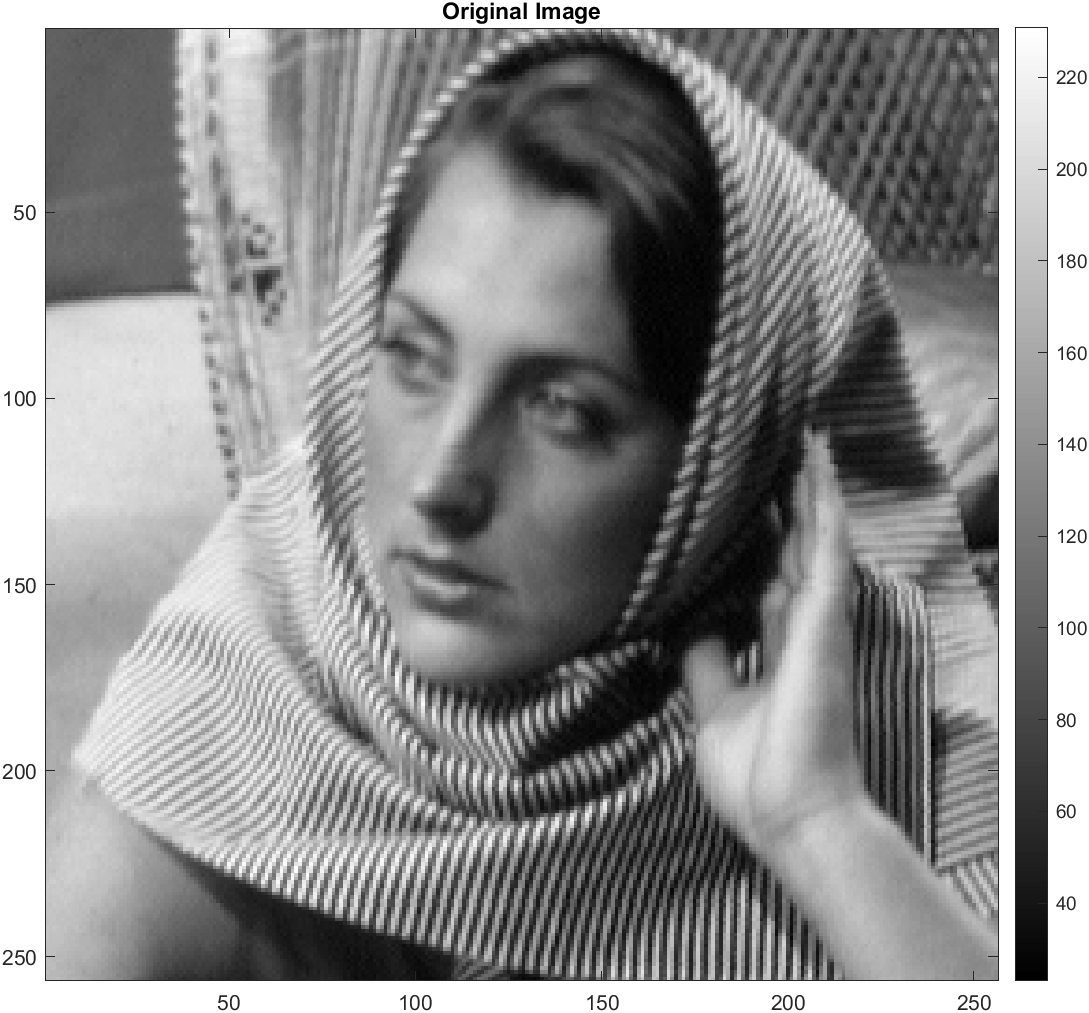
\includegraphics[scale=0.5]{barbara.png}  % change scale factor to re-size the image.
  % give a caption.
  \caption{Barbara image}
  % a label to refer to the figure
  \label{fig:1}
\end{figure}
RMSE = $||X(:) - \hat{X(:)}||_2/||X(:)||_2$
\subsection*{2.a}
\textbf{Root Mean square error due to noise: 0.0146}\\
\textbf{Root Mean square error after reconstruction: 0.0135}
\begin{figure}[H]
  % will center the figure.
  \centering
  % include graphics (can include eps, jpg, pdf ...)
  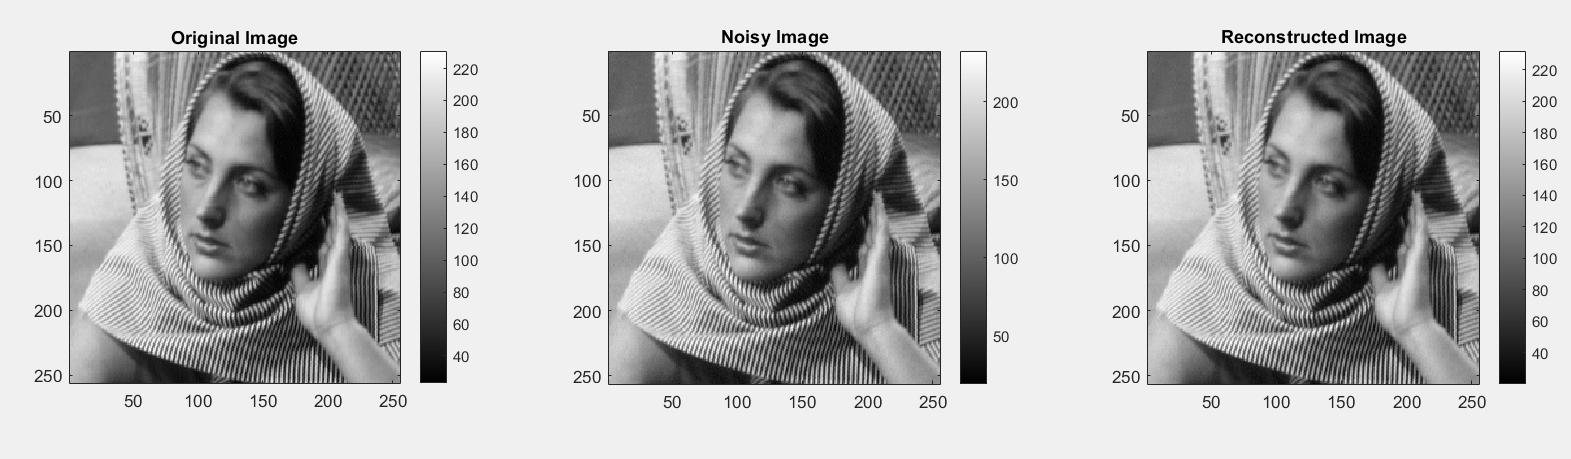
\includegraphics[scale=0.4]{fig2a.png}  % change scale factor to re-size the image.
  % give a caption.
  \caption{All figures at one place for easier observation}
  % a label to refer to the figure
  \label{fig:2}
\end{figure}
\clearpage
\subsection*{2.b}
\textbf{Root Mean square error after reconstruction: 0.406}
\begin{figure}[H]
  % will center the figure.
  \centering
  % include graphics (can include eps, jpg, pdf ...)
  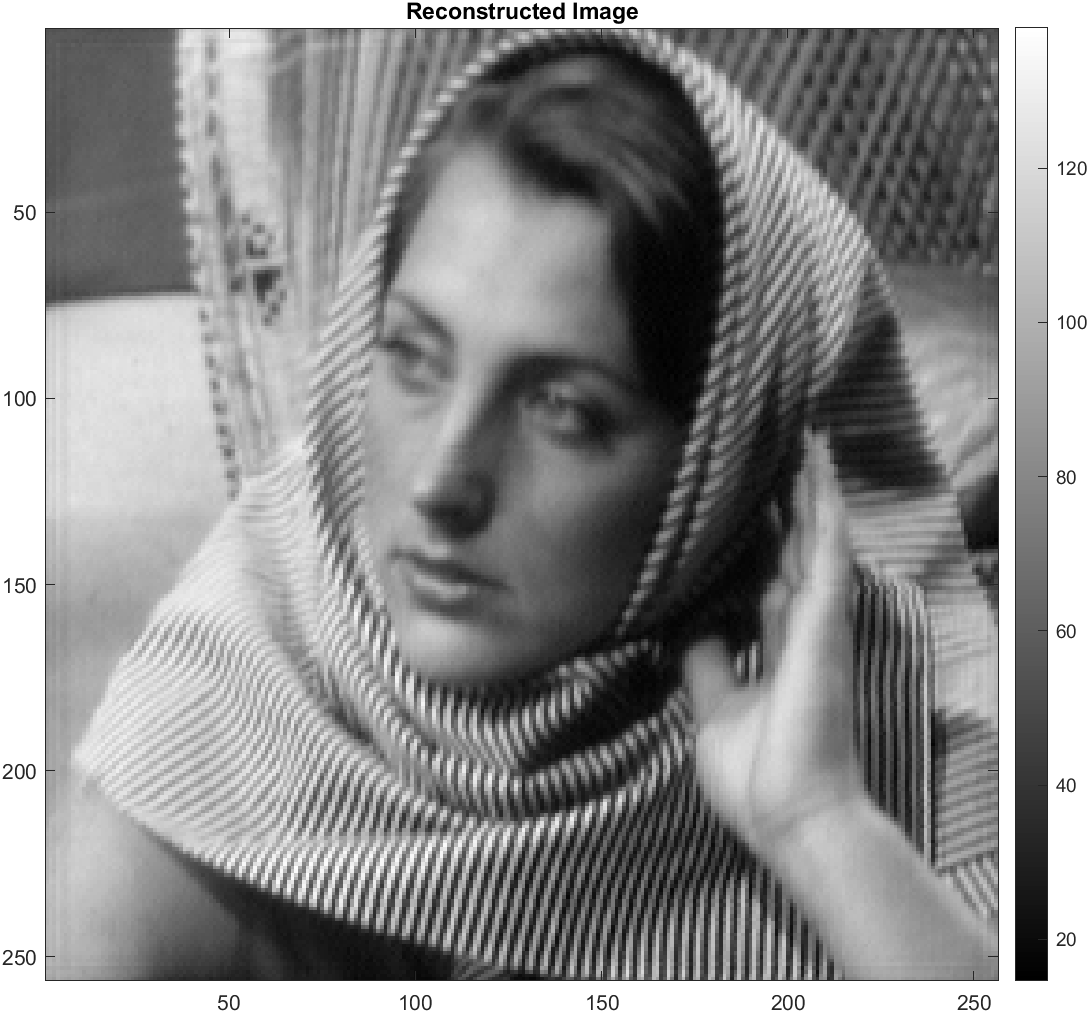
\includegraphics[scale=0.4]{rec_dct.png}  % change scale factor to re-size the image.
  % give a caption.
  \caption{Reconstructed Barbara Image using DCT as the sparsing basis}
  % a label to refer to the figure
  \label{fig:3}
\end{figure}
\subsection*{2.c}
\textbf{Root Mean square error after reconstruction: 0.5678}\\
This code took almost 1.5hrs to compile even when the number of iterations for ista was 20.
\begin{figure}[H]
  % will center the figure.
  \centering
  % include graphics (can include eps, jpg, pdf ...)
  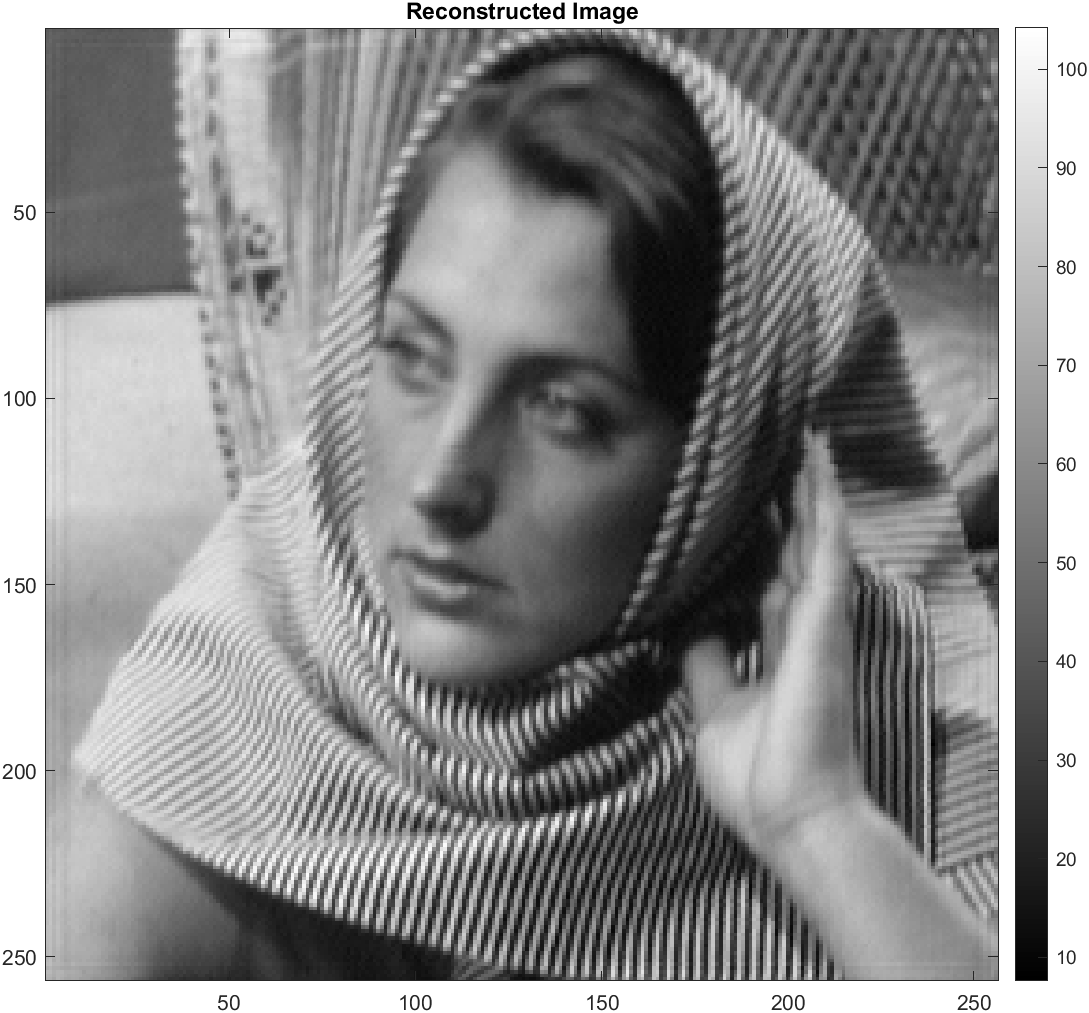
\includegraphics[scale=0.4]{rec_dwt.png}  % change scale factor to re-size the image.
  % give a caption.
  \caption{Reconstructed Barbara Image using DWT as the sparsing basis}
  % a label to refer to the figure
  \label{fig:4}
\end{figure}
\subsection*{2.d}
\textbf{Root Mean square error after reconstruction: 0.853}\\
\begin{figure}[H]
  % will center the figure.
  \centering
  % include graphics (can include eps, jpg, pdf ...)
  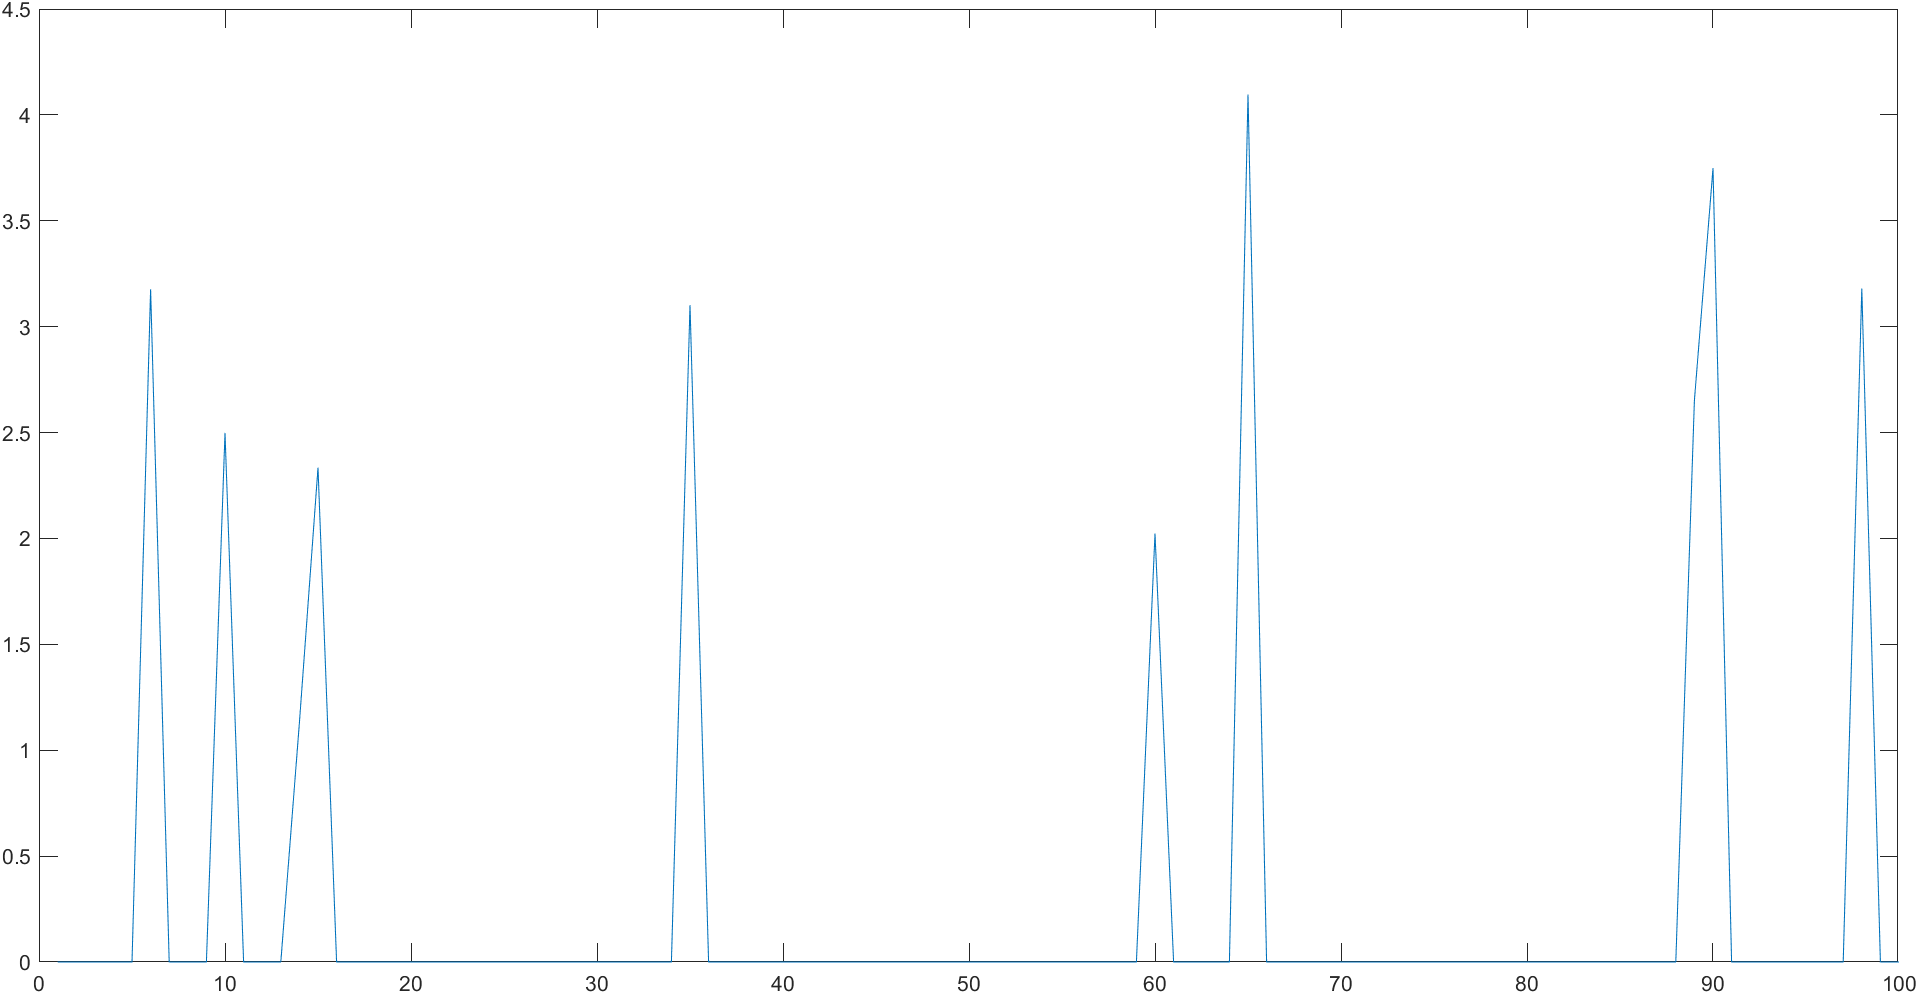
\includegraphics[scale=0.35]{orig_signal.png}  % change scale factor to re-size the image.
  % give a caption.
  \caption{Original sparse signal}
  % a label to refer to the figure
  \label{fig:5}
\end{figure}
\begin{figure}[H]
  % will center the figure.
  \centering
  % include graphics (can include eps, jpg, pdf ...)
  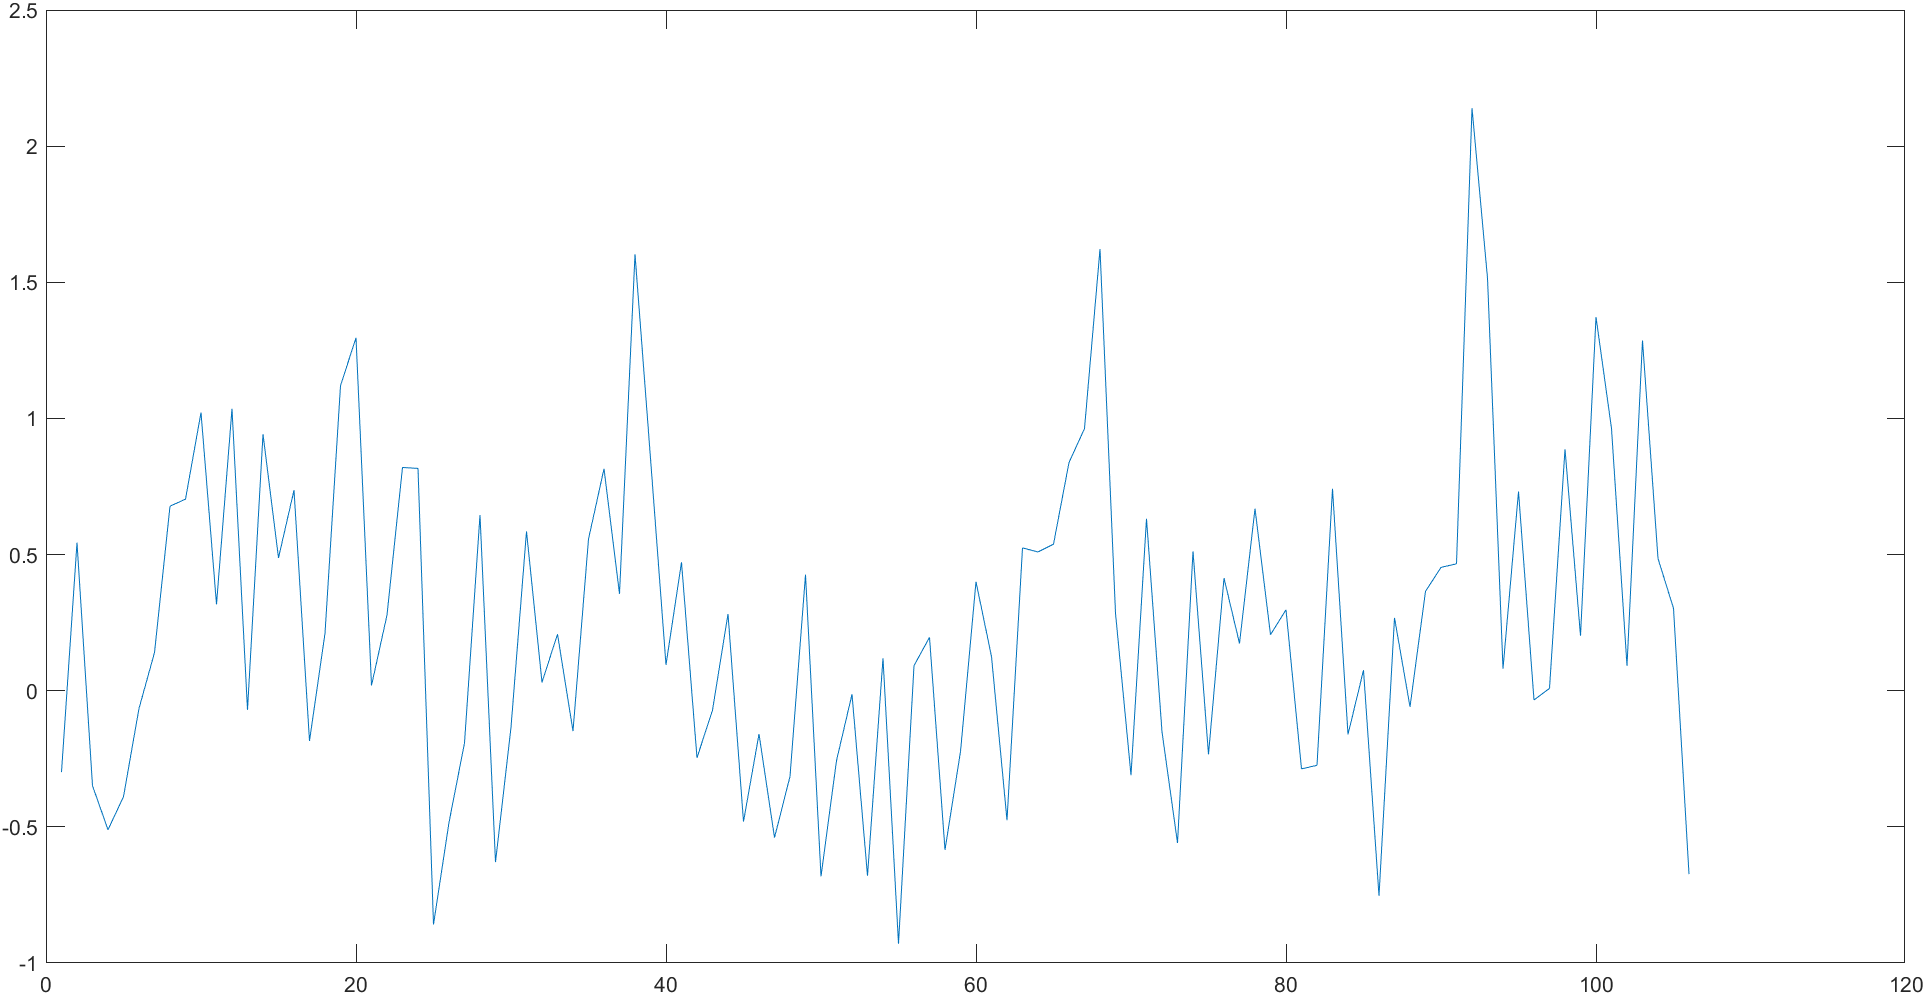
\includegraphics[scale=0.35]{noisy_conv_signal.png}  % change scale factor to re-size the image.
  % give a caption.
  \caption{Noisy Convolved Signal}
  % a label to refer to the figure
  \label{fig:6}
\end{figure}
\begin{figure}[H]
  % will center the figure.
  \centering
  % include graphics (can include eps, jpg, pdf ...)
  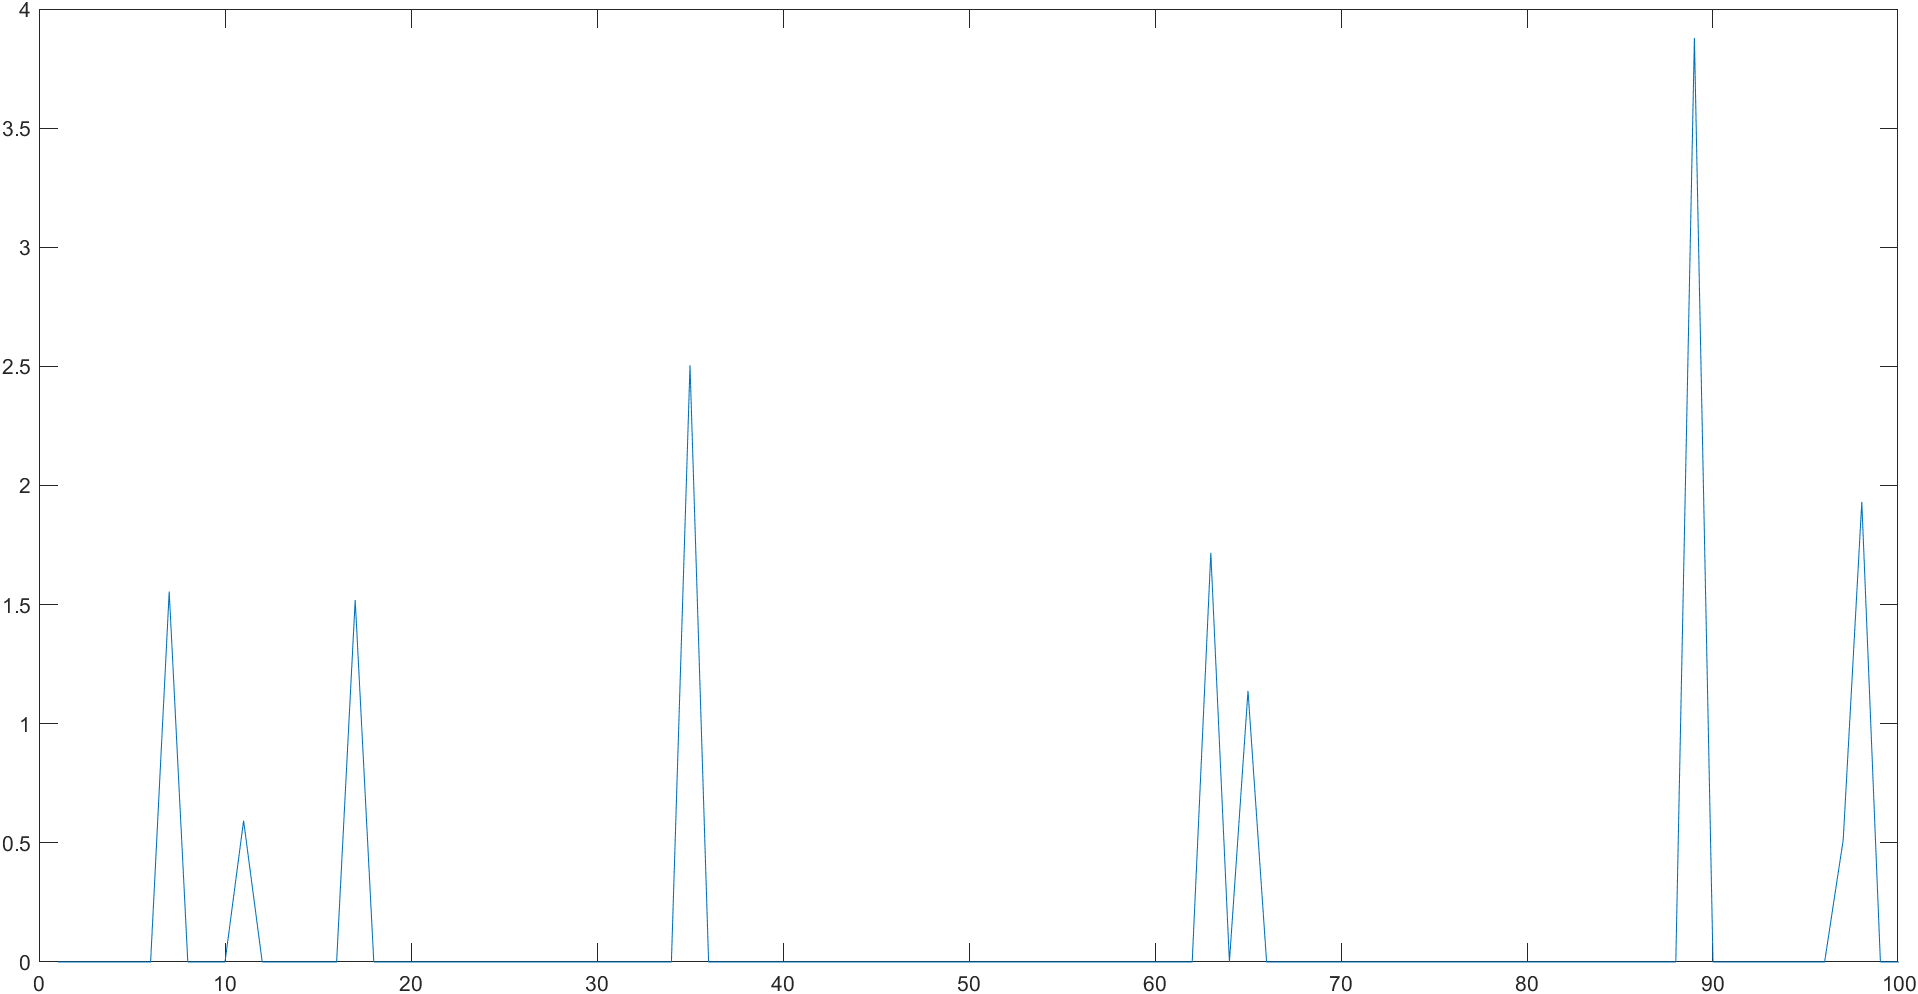
\includegraphics[scale=0.35]{rec_signal.png}  % change scale factor to re-size the image.
  % give a caption.
  \caption{Reconstructed Signal}
  % a label to refer to the figure
  \label{fig:7}
\end{figure}

\section*{Question 3}
\subsection*{3.a}
The oracular solution will be nothing but the solution of the linear equation
$$\boldsymbol{y} = \boldsymbol{\Phi_S} \boldsymbol{x_S}$$
which is nothing but
$$\boldsymbol{\tilde{x}} = \boldsymbol{\Phi_S^\dagger}\boldsymbol{y}$$
\subsection*{3.b}
\begin{eqnarray*}
\norm{\boldsymbol{\tilde{x}} - \boldsymbol{x}}_2 &=& \norm{\boldsymbol{\Phi_S^\dagger y - x}}_2\\
&=&\norm{\boldsymbol{\Phi_S^\dagger}(\boldsymbol{\Phi x - \eta}) - \boldsymbol{x}}_2\\
&=& \norm{\boldsymbol{\Phi_S^\dagger \eta}}_2 \leq \norm{\boldsymbol{\Phi_S^\dagger}}_2 \norm{\boldsymbol{\eta}}_2
\end{eqnarray*}
\subsection*{3.c}
We know that if $\lambda_i$ are the non-zero singular values of $\boldsymbol{\Phi}$, then the singular values of $\boldsymbol{\Phi_S^\dagger}$ will be $\lambda_i^{-1}$. Also, if the eigen values of $\boldsymbol{\Phi}$ are denoted as $e_i$, then we know $\lambda_i = \sqrt{e_i}$.\\
As $\boldsymbol{\Phi}$ satisfies restricted isometry property of order $2k$, we have
$$(1 - \delta_{2k}) \norm{\boldsymbol{x}}_2^2 \leq \norm{\boldsymbol{\Phi x}}_2^2 \leq (1 + \delta_{2k}) \norm{\boldsymbol{x}}_2^2$$
Re-writing $\norm{A}_2^2 = A^T A$, we can say that 
$$1 - \delta_{2k} \leq e_i \leq 1 + \delta_{2k}$$
which is equivalent to
$$\frac{1}{\sqrt{1 + \delta_{2k}}} \leq \frac{1}{\lambda_i} \leq \frac{1}{\sqrt{1 - \delta_{2k}}}$$
Hence we can say that the largest singular value of $\boldsymbol{\Phi_S^\dagger}$ lies between $\frac{1}{\sqrt{1 + \delta_{2k}}}$ and $\frac{1}{\sqrt{1 - \delta_{2k}}}$
\subsection*{3.d}
From Noisy recovery theorem, we have
$$\norm{x^* - x}_2 \leq C_0 k^{-1/2} \norm{x - \tilde{x}}_1 + C_1 \epsilon$$
We know that for a $2k$ sparse vector $x - \tilde{x}$, we have
$$\norm{x - \tilde{x}}_1 \leq \sqrt{2k} \norm{x - \tilde{x}}_2$$
Hence, we have
$$\norm{x^* - x}_2 \leq \sqrt{2} C_0 \norm{x - \tilde{x}}_2 + C_1 \epsilon$$
But we have
$$\norm{x - \tilde{x}}_2 \leq \frac{\epsilon}{\sqrt{1 - \delta_{2k}}}$$
Hence, we will have
$$\norm{x^* - x}_2 \leq C_2 \frac{\epsilon}{\sqrt{1 - \delta_{2k}}}$$
where 
$$C_2 = C_0 \sqrt{2}+ C_1 \sqrt{1 - \delta_{2k}}$$
which is a constant factor.

\section*{Question 4}
As derived in lecture, we have the following relationship:
\begin{equation*}
    \delta_s = max\{1-\lambda_{min}, \lambda_{max}-1\}
\end{equation*}
where, $\lambda_{max}$ and $\lambda_{min}$ the maximum and minimum eigenvalues of the matrix
$(\boldsymbol{A_{\Gamma}})^T(\boldsymbol{A_{\Gamma}})$ over all sets $\Gamma$. Here, $\Gamma$ is an index set of columns of $\boldsymbol{A}$ whose cardinality is less than or equal to s(sparsity of the vector $\theta$) and $\boldsymbol{A_{\Gamma}}$ denotes a sub matrix obtained by retaining those columns of $\boldsymbol{A}$ whose index belongs to $\Gamma$. \\
Now let us take $t\geq s$. In this case all the possible sets whose cardinality is less than $t$ will be covered by $\Gamma$. Thus, $\Gamma$ will cover sets with cardinality less than or equal to $s$ also. When we take maximum and minimum Eigen-values over all such sets then we have the following two relationships:
\begin{align*}
    \lambda_{s, max} \leq \lambda_{t, max}; \ \ \lambda_{t, min} \leq \lambda_{s, min}
\end{align*}
which is obvious as searching for maximum and minimum values over a larger set will give us more rigorous values. Thus we have:
\begin{align*}
    \lambda_{s, max}-1 \leq \lambda_{t, max}-1; \ \ 1-\lambda_{t, min} \geq 1-\lambda_{s, min}
\end{align*}
which finally gives:
\begin{equation*}
    max\{1-\lambda_{t, min}, \lambda_{t, max}-1\} \geq max\{1-\lambda_{s, min}, \lambda_{s, max}-1\}
\end{equation*}
Thus, we have $\delta_t \geq \delta_s$ for $t \geq s$.

\section*{Question 5}
\begin{itemize}
\item Title: Boolean Compressed Sensing and
Noisy Group Testing
\item Link: \href{https://arxiv.org/pdf/0907.1061.pdf}{https://arxiv.org/pdf/0907.1061.pdf}
\item Objective Function:\\
Here, we try to maximize the likelihood of decoder which in essense minimizes the error probability. For $N$ items and a defective set of size $K$, the decoder goes through all $N \choose K$ possible sets of size $K$ and chooses the set that is most likely. If we denote the tests' outcomes as $Y^T$, we choose $\omega^*$ for which 
$$p(Y^T | \boldsymbol{X}_{S_{\omega^*}}) > p(Y^T|\boldsymbol{X}_{S_{\omega}}); \:\:\: \forall \omega \neq \omega^* $$
Here
\begin{itemize}
	\item $N$ is the total number of items, $k$ is the known number of defectives (or positive items), $p$ denotes the
	probability that an item is part of a given test, and $T$ is the total number of tests
	\item Codewords: For the $j$-th term, $X_j^T$ is a binary vector $\in \{0,1\}^T$, with the $t$-th entry $X_j(t) = 1$ if the $j$-th item is pooled in test $t$, and 0 otherwise. Following an information theoretic convention, we call it the $j$-th
	codeword. The observation vector $Y^T$ is a binary vector of length $T$, with entries equal to 1 for the tests with positive outcome. Similarly $Y(t)$ denotes the $t$-th component of the vector $Y^T$.
	\item $\boldsymbol{X} \in \{0, 1\}^{N \times T}$ is the measurement matrix, or the codebook, which is a collection of $N$ codewords defining the pool design, i.e., the assignment of items to tests.
	$$\boldsymbol{X} = [X_1^T; X_2^T; \ldots; X_N^T]$$
	\item Given a subset $S \subset \{1, 2, \ldots N\}$ with cardinality $|S|$, the matrix $\boldsymbol{X}_S$ is an $|S|\times T$ matrix formed from the rows indexed by $S$. In other words, $\boldsymbol{X}_S$ denotes the codewords (each of length $T$) corresponding to the items in $S$. Similarly, $X_S$ denotes a vector, whose components are restricted to the set of components indexed by $S$. Thus, $X_S$ is a column of the matrix $\boldsymbol{X}_S$. When indexing by test is needed, $X_S(t)$ is used to specifically denote the $t$-th column of the matrix $\boldsymbol{X}_S$, and $X_j(t)$ is the $t$-th component of the vector $X_j^T$.
	\item Index the different sets of items of size $K$ as $S_\omega$ with index $\omega$. Since there are $N$ items in total, there are $N \choose K$ such sets, hence
	$$\omega \in \mathcal{I} = \bigg\{1, 2, \ldots, {N\choose K} \bigg\}$$
\end{itemize}
\item Differences between Tapestry and the proposed method:
\begin{enumerate}
\item  Tapestry models the task from a linear algebra perspective whereas the proposed method models the task from an Information Theory perspective making use of channel coding concepts and probability and random processes.
\item Tapestry solves a constrained convex optimization problem whereas the proposed method solves an un-constrained optimization problem.
\item In Tapestry pooling, we model noise as a Poisson random variable whereas in the proposed method they model it as a Bernoulli random variable.
\end{enumerate}
\end{itemize}

\section*{Question 6}
Let $\boldsymbol{x_{min}}$ be the vector which minimizes the lasso cost function. Thus we have:
\begin{equation*}
    J'(\boldsymbol{x})|_{\boldsymbol{x = x_{min}}} = 2||\boldsymbol{y-\Phi x}||_2|_{\boldsymbol{x = x_{min}}}\frac{d||\boldsymbol{y-\Phi x}||_2}{d\boldsymbol{x}}|_{\boldsymbol{x = x_{min}}}+\lambda\frac{d||\boldsymbol{x}||_1}{d\boldsymbol{x}}|_{\boldsymbol{x = x_{min}}}=0
\end{equation*}
As hinted by the question let $||\boldsymbol{y-\Phi x}||_2|_{\boldsymbol{x = x_{min}}} = \epsilon'$. Thus, the condition finally becomes:
\begin{equation}
    -\frac{2}{\lambda}\epsilon'\frac{d||\boldsymbol{y-\Phi x}||_2}{d\boldsymbol{x}}|_{\boldsymbol{x = x_{min}}} = \frac{d||\boldsymbol{x}||_1}{d\boldsymbol{x}}|_{\boldsymbol{x = x_{min}}}
\end{equation}
Now we have three cases:\\
\textbf{Case1:} A global minima was found for $\boldsymbol{||x||_1}$ and $\epsilon' = 0$. In this case exact reconstruction was possible as $||\boldsymbol{y-\Phi x_{min}}||_2 = 0$ and thus this solution would also satisfy the P1 problem and we can have $\epsilon$ as any positive value. \\
\textbf{Case2:} A global minima was found for $\boldsymbol{||x||_1}$ and $\frac{d||\boldsymbol{y-\Phi x}||_2}{d\boldsymbol{x}}|_{\boldsymbol{x = x_{min}}} = 0$. In this case exact reconstruction was not possible but we achieved the best possible reconstruction as global minima for $||\boldsymbol{y-\Phi x}||_2$ was also achieved. For this case we can set $\epsilon$ as any value greater than $\epsilon'$. Thus, when solving P1 problem with such constraint, we will be guaranteed that we are searching and finally finding the best possible solution and reconstruction. Therefore, solution to the lasso problem would also solve the P1 problem given that $\epsilon \geq \epsilon'$. \\
\textbf{Case3:} When both sides of the Eq(28) were non-zero. This means that the cost function is minimized at $\boldsymbol{x = x_{min}}$ which is not the global minimum for our function in the P1 problem. The P1 problem is:
\begin{equation*}
    min_{\boldsymbol{x}}||\boldsymbol{x}||_1 \ s.t\ ||\boldsymbol{y-\Phi x}||_2 \leq \epsilon
\end{equation*}
We know that the solution to such constrained optimization problem lies at the boundary which is explained clearly in the fig. given below.
\begin{figure}[H]
  % will center the figure.
  \centering
  % include graphics (can include eps, jpg, pdf ...)
  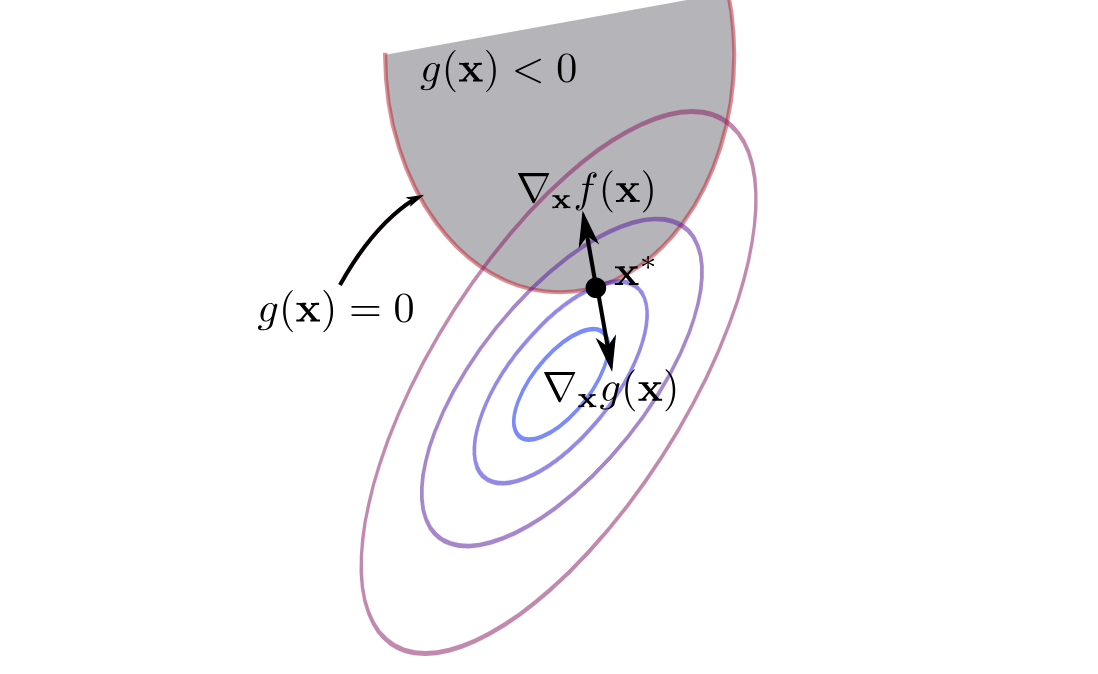
\includegraphics[scale=0.7]{fig6.png}  % change scale factor to re-size the image.
  % give a caption.
  \caption{Figure taken from \href{http://www.juyang.co/numerical-optimization-in-machine-learning-iii-constrained-optimization/}{here}}
  % a label to refer to the figure
  \label{fig:9}
\end{figure}
Thus, we can apply Lagrangian Multiplier method to solve the optimization, which gives:
\begin{equation*}
    c\frac{d(||\boldsymbol{y-\Phi x}||_2-\epsilon)}{d\boldsymbol{x}} + \frac{d||\boldsymbol{x}||_1}{d\boldsymbol{x}} = 0
\end{equation*}
where c is Lagrangian Multiplier constant and $\epsilon$ is some constant whose derivative is zero. Looking at this equation and the Eq(28) we see that if we put $\epsilon = \epsilon'$ then $c$ will become $-\frac{2}{\lambda}\epsilon'$ and we will be solving the same set of equations to get the elements of vector $\boldsymbol{x}$. Hence, we have proved the existence of the constraint parameter $\epsilon$ such that the solution corresponding to lasso will be solution for P1 problem also.\\
Therefore, we see for any case there exist some $\epsilon$ such that the solution to lasso problem will also be a solution to P1 problem.
\end{document}P of order $2s$, we have
$$\norm{\Phi h_{T_0 \cup T_1}}_2 \leq \sqrt{1 + \delta_{2s}} \, \norm{ h_{T_0 \cup T_1}}_2$$
Using the above two inequalities in (14), we have
\begin{equation}
	|\langle \Phi h_{T_0 \cup T_1}, \Phi h\rangle| \leq \norm{\Phi  h_{T_0 \cup T_1}}_2 \, \norm{\Phi h}_2 \leq 	2\epsilon \sqrt{1 + \delta_{2s}} \, \norm{ h_{T_0 \cup T_1}}_2
\end{equation}
\subsection*{1.10}
Lemma 2.1 from the paper states
$$|\langle \Phi x, \Phi x' \rangle | \leq \delta_{s + s'}\, \norm{x}_2 \norm{x'}_2$$
for all $x, x'$ supported on disjoint subsets $T, T' \subset \{1, 2, \ldots, n\}$ with $|T| \leq s, |T'| \leq s'$
Using this lemma for $x = h_{T_0}$ and $x' = h_{T_j}$, we have
\begin{equation}
|\langle \Phi h_{T_0}, \Phi h_{T_j}\rangle | \leq \delta_{2s} \, \norm{h_{T_0}}_2 \norm{h_{T_j}}_2
\end{equation}
\subsection*{1.11}
We know that for two positive real numbers $a$ and $b$, the QM-AM inequality is as follows:
$$\frac{a + b}{2} \leq \sqrt{\frac{a^2 + b^2}{2}}$$
Taking $a = \norm{h_{T_0}}_2$ and $b = \norm{h_{T_1}}_2$ and substituting in the above inequality, we get
\begin{equation}
\norm{h_{T_0}}_2 + \norm{h_{T_1}}_2 \leq \sqrt{2} \:\sqrt{\norm{h_{T_0}}_2^2 + \norm{h_{T_1}}_2^2} = \sqrt{2}\, \norm{h_{T_0 \cup T_1}}_2
\end{equation}
as $T_0$ and $T_1$ are disjoint.
\subsection*{1.12}
By replacing $T_0$ with $T_1$ in inequality (16) and adding both, we get
$$|\langle \Phi h_{T_0}, \Phi h_{T_j}\rangle | + |\langle \Phi h_{T_1}, \Phi h_{T_j}\rangle | \leq \delta_{2s} (\norm{h_{T_0}}_2 + \norm{h_{T_1}}_2) \norm{h_{T_{j}}}$$
Making use of triangle inequality for the LHS of above inequality, we get
$$|\langle \Phi h_{T_0} + \Phi h_{T_1}, \Phi h_{T_j}\rangle | \leq \delta_{2s} (\norm{h_{T_0}}_2 + \norm{h_{T_1}}_2) \norm{h_{T_{j}}}$$
Replacing $\Phi h_{T_0} + \Phi h_{T_1} = \Phi h_{T_0 \cup T_1}$ and above inequalities for $j \geq 2$, we get
$$\sum \limits_{j \geq 2} |\langle \Phi h_{T_0 \cup T_1}, \Phi h_{T_j}\rangle |\leq \delta_{2s} (\norm{h_{T_0}}_2 + \norm{h_{T_1}}_2) \, \bigg(\sum \limits_{j \geq 2} \norm{h_{T_j}}_2\bigg)$$
Again making use of triangle inequality for the LHS of the above inequality, we get
$$\bigg|\bigg\langle \Phi h_{T_0 \cup T_1}, \sum_{j \geq 2} \Phi h_{T_j}\bigg\rangle \bigg| \leq \delta_{2s} (\norm{h_{T_0}}_2 + \norm{h_{T_1}}_2) \, \bigg(\sum \limits_{j \geq 2} \norm{h_{T_j}}_2\bigg)$$
Finally, using (17), we finally have
\begin{equation}
\bigg|\bigg\langle \Phi h_{T_0 \cup T_1}, \sum_{j \geq 2} \Phi h_{T_j}\bigg\rangle \bigg| \leq \delta_{2s} \, \sqrt{2}\,\norm{h_{T_0 \cup T_1}} \, \bigg(\sum \limits_{j \geq 2} \norm{h_{T_j}}_2\bigg)
\end{equation}
Now, using the fact that $\Phi h = \Phi h_{T_0 \cup T_1} + \sum_{j \geq 2} \Phi h_{T_j}$ in the inequality (15) above, we get
$$\bigg|\bigg\langle \Phi h_{T_0 \cup T_1}, \Phi h_{T_0 \cup T_1} + \sum_{j \geq 2} \Phi h_{T_j}\bigg\rangle \bigg| \leq 	2\epsilon \sqrt{1 + \delta_{2s}} \, \norm{ h_{T_0 \cup T_1}}_2$$
Using the linearity property of inner product, we have
\begin{equation}
	\bigg|\norm{\Phi h_{T_0 \cup T_1}}_2^2 + \bigg\langle \Phi h_{T_0 \cup T_1}, \sum_{j \geq 2} \Phi h_{T_j}\bigg\rangle \bigg| \leq 	2\epsilon \sqrt{1 + \delta_{2s}} \, \norm{ h_{T_0 \cup T_1}}_2
\end{equation}
Now, adding the inequalities (18) and (19), we get
\begin{eqnarray*}
\bigg|\norm{\Phi h_{T_0 \cup T_1}}_2^2 + \bigg\langle \Phi h_{T_0 \cup T_1}, \sum_{j \geq 2} \Phi h_{T_j}\bigg\rangle \bigg| + \bigg|\bigg\langle \Phi h_{T_0 \cup T_1}, \sum_{j \geq 2} \Phi h_{T_j}\bigg\rangle \bigg| &\leq& 	2\epsilon \sqrt{1 + \delta_{2s}} \, \norm{ h_{T_0 \cup T_1}}_2 + \\ 
&& \delta_{2s} \, \sqrt{2}\,\norm{h_{T_0 \cup T_1}} \, \bigg(\sum \limits_{j \geq 2} \norm{h_{T_j}}_2\bigg)
\end{eqnarray*}
We know from the triangle inequality that 
$$\norm{\Phi h_{T_0 \cup T_1}}_2^2 \leq \bigg|\norm{\Phi h_{T_0 \cup T_1}}_2^2 + \bigg\langle \Phi h_{T_0 \cup T_1}, \sum_{j \geq 2} \Phi h_{T_j}\bigg\rangle \bigg| + \bigg|- \bigg\langle \Phi h_{T_0 \cup T_1}, \sum_{j \geq 2} \Phi h_{T_j}\bigg\rangle \bigg|$$
Using this, we finally have,
\begin{equation}
\norm{\Phi h_{T_0 \cup T_1}}_2^2 \leq \norm{ h_{T_0 \cup T_1}}_2 \, \bigg(2\epsilon \sqrt{1 + \delta_{2s}} + \sqrt{2}\,\delta_{2s}\,\sum \limits_{j \geq 2} \norm{h_{T_j}}_2\bigg)
\end{equation}
From the restricted isometry property, we have
$$(1 - \delta_{2s})\, \norm{h_{T_0 \cup T_1}}_2^2 \leq \norm{\Phi h_{T_0 \cup T_1}}_2^2$$
Hence, we have
\begin{equation}
(1 - \delta_{2s})\, \norm{h_{T_0 \cup T_1}}_2^2 \leq \norm{\Phi h_{T_0 \cup T_1}}_2^2 \leq
\norm{ h_{T_0 \cup T_1}}_2 \, \bigg(2\epsilon \sqrt{1 + \delta_{2s}} + \sqrt{2}\,\delta_{2s}\,\sum \limits_{j \geq 2} \norm{h_{T_j}}_2\bigg) 
\end{equation}
\subsection*{1.13}
By combining the inequality (6) with RHs of (21), we have
$$\norm{ h_{T_0 \cup T_1}}_2 \, \bigg(2\epsilon \sqrt{1 + \delta_{2s}} + \sqrt{2}\,\delta_{2s}\,\sum \limits_{j \geq 2} \norm{h_{T_j}}_2\bigg) \leq \norm{h_{T_0 \cup T_1}}_2 \bigg(2\epsilon \sqrt{1 + \delta_{2s}} + \sqrt{2}\delta_{2s} \, s^{-1/2} \norm{h_{T_0^c}}_1\bigg)$$
Using the above inequality with (21), we have
$$(1 - \delta_{2s})\norm{h_{T_0 \cup T_1}}_2^2 \leq \norm{h_{T_0 \cup T_1}}_2 \bigg(2\epsilon \sqrt{1 + \delta_{2s}} + \sqrt{2}\delta_{2s} \, s^{-1/2} \norm{h_{T_0^c}}_1\bigg)$$
On simplifying the above inequality, we get
\begin{equation}
\norm{h_{T_0 \cup T_1}}_2 \leq \alpha \epsilon + \rho s^{-1/2} \norm{h_{T_0^c}}_1, \:\:\: \alpha \equiv \frac{2 \sqrt{1 + \delta_{2s}}}{1 - \delta_{2s}}, \rho \equiv \frac{\sqrt{2}\delta_{2s}}{1 - \delta_{2s}}
\end{equation}
\subsection*{1.14}
We now conclude from (22) and (12) that 
$$\norm{h_{T_0 \cup T_1}}_2 \leq \alpha \epsilon + \rho s^{-1/2}\norm{h_{T_0}}_1 + 2\rho e_0 \leq \alpha \epsilon + \rho \norm{h_{T_0}}_2 + 2\rho e_0$$
As $T_0$ and $T_1$ are disjoint and $h_{T_0}$ and $h_{T_1}$ are both $s$ sparse, we can say that 
$$\norm{h_{T_0}}_2 \leq \norm{h_{T_0} + h_{T_1}}_2 = \norm{h_{T_0 \cup T_1}}_2$$
Using this in the above inequality, we get
$$\norm{h_{T_0 \cup T_1}}_2 \leq \alpha \epsilon + \rho \norm{h_{T_0 \cup T_1}}_2 + 2 \rho e_0$$
On simplifying, we get
\begin{equation}
\norm{h_{T_0 \cup T_1}}_2 \leq (1 - \rho)^{-1} \, (\alpha \epsilon + 2\rho e_0)
\end{equation}
\subsection*{1.15}
We can write $h$ as
$$h = h_{T_0 \cup T_1} + h_{(T_0 \cup T_1)^c}$$
Hence, by triangle inequality, we have
$$\norm{h}_2 \leq \norm{h_{T_0 \cup T_1}}_2 + \norm{h_{(T_0 \cup T_1)^c}}_2$$
But from (13), we know that
$$\norm{h_{(T_0 \cup T_1)^c}}_2 \leq \norm{h_{T_0}}_2 + 2e_0 \leq \norm{h_{T_0 \cup T_1}} + 2e_0$$
Combining the above two inequalities, we get
\begin{equation}
\norm{h}_2 \leq 2 \norm{h_{T_0}}_2 + 2e_0
\end{equation}
Now combining (24) with (23) we get
\begin{equation}
\norm{h}_2 \leq 2 \norm{h_{T_0}}_2 + 2e_0 \leq 2\,(1 - \rho)^{-1}\,\big(\alpha \epsilon + (1 + \rho)e_0\big)
\end{equation}
\subsection*{1.16}
We know that
$$\norm{h_{T_0}}_1 \leq \rho \norm{h_{T_0^c}}_1$$
Adding $\norm{h_{T_0^c}}_1$ on both sides, we get
\begin{equation}
\norm{h}_1 \leq (1 + \rho) \norm{h_{T_0^c}}_1
\end{equation}
Using the result 
$$\norm{h_{T_0^c}}_1 \leq 2(1 - \rho)^{-1} \norm{x_{T_0^c}}_1$$
in (26), we get
\begin{equation}
\norm{h}_1 \leq 2(1+\rho)(1-\rho)^{-1} \norm{x_{T_0^c}}_1
\end{equation}
\newpage
\section*{Question 3}
\subsection*{3.a}
The oracular solution will be nothing but the solution of the linear equation
$$\boldsymbol{y} = \boldsymbol{\Phi_S} \boldsymbol{x_S}$$
which is nothing but
$$\boldsymbol{\tilde{x}} = \boldsymbol{\Phi_S^\dagger}\boldsymbol{y}$$
\subsection*{3.b}
\begin{eqnarray*}
\norm{\boldsymbol{\tilde{x}} - \boldsymbol{x}}_2 &=& \norm{\boldsymbol{\Phi_S^\dagger y - x}}_2\\
&=&\norm{\boldsymbol{\Phi_S^\dagger}(\boldsymbol{\Phi x - \eta}) - \boldsymbol{x}}_2\\
&=& \norm{\boldsymbol{\Phi_S^\dagger \eta}}_2 \leq \norm{\boldsymbol{\Phi_S^\dagger}}_2 \norm{\boldsymbol{\eta}}_2
\end{eqnarray*}
\subsection*{3.c}
We know that if $\lambda_i$ are the non-zero singular values of $\boldsymbol{\Phi}$, then the singular values of $\boldsymbol{\Phi_S^\dagger}$ will be $\lambda_i^{-1}$. Also, if the eigen values of $\boldsymbol{\Phi}$ are denoted as $e_i$, then we know $\lambda_i = \sqrt{e_i}$.\\
As $\boldsymbol{\Phi}$ satisfies restricted isometry property of order $2k$, we have
$$(1 - \delta_{2k}) \norm{\boldsymbol{x}}_2^2 \leq \norm{\boldsymbol{\Phi x}}_2^2 \leq (1 + \delta_{2k}) \norm{\boldsymbol{x}}_2^2$$
Re-writing $\norm{A}_2^2 = A^T A$, we can say that 
$$1 - \delta_{2k} \leq e_i \leq 1 + \delta_{2k}$$
which is equivalent to
$$\frac{1}{\sqrt{1 + \delta_{2k}}} \leq \frac{1}{\lambda_i} \leq \frac{1}{\sqrt{1 - \delta_{2k}}}$$
Hence we can say that the largest singular value of $\boldsymbol{\Phi_S^\dagger}$ lies between $\frac{1}{\sqrt{1 + \delta_{2k}}}$ and $\frac{1}{\sqrt{1 - \delta_{2k}}}$
\subsection*{3.d}
From Noisy recovery theorem, we have
$$\norm{x^* - x}_2 \leq C_0 k^{-1/2} \norm{x - \tilde{x}}_1 + C_1 \epsilon$$
We know that for a $2k$ sparse vector $x - \tilde{x}$, we have
$$\norm{x - \tilde{x}}_1 \leq \sqrt{2k} \norm{x - \tilde{x}}_2$$
Hence, we have
$$\norm{x^* - x}_2 \leq \sqrt{2} C_0 \norm{x - \tilde{x}}_2 + C_1 \epsilon$$
But we have
$$\norm{x - \tilde{x}}_2 \leq \frac{\epsilon}{\sqrt{1 - \delta_{2k}}}$$
Hence, we will have
$$\norm{x^* - x}_2 \leq C_2 \frac{\epsilon}{\sqrt{1 - \delta_{2k}}}$$
where 
$$C_2 = C_0 \sqrt{2}+ C_1 \sqrt{1 - \delta_{2k}}$$
which is a constant factor.
\section*{Question 5}
\begin{itemize}
\item Title: Boolean Compressed Sensing and
Noisy Group Testing
\item Link: \href{https://arxiv.org/pdf/0907.1061.pdf}{https://arxiv.org/pdf/0907.1061.pdf}
\item Objective Function:\\
Here, we try to maximize the likelihood of decoder which in essense minimizes the error probability. For $N$ items and a defective set of size $K$, the decoder goes through all $N \choose K$ possible sets of size $K$ and chooses the set that is most likely. If we denote the tests' outcomes as $Y^T$, we choose $\omega^*$ for which 
$$p(Y^T | \boldsymbol{X}_{S_{\omega^*}}) > p(Y^T|\boldsymbol{X}_{S_{\omega}}); \:\:\: \forall \omega \neq \omega^* $$
Here
\begin{itemize}
	\item $N$ is the total number of items, $k$ is the known number of defectives (or positive items), $p$ denotes the
	probability that an item is part of a given test, and $T$ is the total number of tests
	\item Codewords: For the $j$-th term, $X_j^T$ is a binary vector $\in \{0,1\}^T$, with the $t$-th entry $X_j(t) = 1$ if the $j$-th item is pooled in test $t$, and 0 otherwise. Following an information theoretic convention, we call it the $j$-th
	codeword. The observation vector $Y^T$ is a binary vector of length $T$, with entries equal to 1 for the tests with positive outcome. Similarly $Y(t)$ denotes the $t$-th component of the vector $Y^T$.
	\item $\boldsymbol{X} \in \{0, 1\}^{N \times T}$ is the measurement matrix, or the codebook, which is a collection of $N$ codewords defining the pool design, i.e., the assignment of items to tests.
	$$\boldsymbol{X} = [X_1^T; X_2^T; \ldots; X_N^T]$$
	\item Given a subset $S \subset \{1, 2, \ldots N\}$ with cardinality $|S|$, the matrix $\boldsymbol{X}_S$ is an $|S|\times T$ matrix formed from the rows indexed by $S$. In other words, $\boldsymbol{X}_S$ denotes the codewords (each of length $T$) corresponding to the items in $S$. Similarly, $X_S$ denotes a vector, whose components are restricted to the set of components indexed by $S$. Thus, $X_S$ is a column of the matrix $\boldsymbol{X}_S$. When indexing by test is needed, $X_S(t)$ is used to specifically denote the $t$-th column of the matrix $\boldsymbol{X}_S$, and $X_j(t)$ is the $t$-th component of the vector $X_j^T$.
	\item Index the different sets of items of size $K$ as $S_\omega$ with index $\omega$. Since there are $N$ items in total, there are $N \choose K$ such sets, hence
	$$\omega \in \mathcal{I} = \bigg\{1, 2, \ldots, {N\choose K} \bigg\}$$
\end{itemize}
\item Differences between Tapestry and the proposed method:
\begin{enumerate}
\item  Tapestry models the task from a linear algebra perspective whereas the porposed method models the task from an Information Theory perspective making use of channel coding concepts and probability and random processes.
\item Tapestry solves a constrained convex optimization problem whereas the proposed method solves an un-constrained optimization problem.
\item In Tapestry pooling, we model noise as a Poisson random variable whereas in the proposed method they model it as a Bernoulli random variable.
\end{enumerate}
\end{itemize}
\end{document}
